\documentclass[12pt]{HomeWork}

%%%%%% ========== 身份信息填写 ========== %%%%%%
\title{数学实验报告}                   %题目
\newcommand{\Class}{数学2xx}               %班级
\newcommand{\Lession}{01}                 %序号 
\newcommand{\Tit}{定积分的近似计算}          %学号
\newcommand{\Num}{2023123456789}          %学号
\author{李奕贝}                            %姓名
%%%%%%%%%%%%%%%%%%%%%%%%%%%%%%%%%%%%%%%%%%%%%%%


%%%%%% ========== 页眉设置 ========== %%%%%%
\fancyhead[C]{\thetitle{}}
\fancyhead[L]{\Class \theauthor{}}
\fancyhead[R]{\today}

\begin{document}
\thispagestyle{empty}

%%%%%% ========== 首页标题 ========== %%%%%%
\begin{center}
    \zihao{3}\heiti \thetitle{}
\end{center}

%%%%%% ========== 基本信息表格 ========== %%%%%%
\noindent
\begin{tabular}{@{}p{0.4\textwidth} p{0.4\textwidth}@{}}
    \quad 实验序号：\Lession & \centering 日期：\today \tabularnewline
\end{tabular}

\vspace{1em}
\noindent
\begin{tabular}{|>{\centering\arraybackslash}p{1.5cm}|
                  >{\centering\arraybackslash}p{2.6cm}|
                  >{\centering\arraybackslash}p{1.5cm}|
                  >{\centering\arraybackslash}p{2.6cm}|
                  >{\centering\arraybackslash}p{1.5cm}|
                  >{\centering\arraybackslash}p{3.4cm}|}
    \hline
    班级 & \Class & 姓名 & \theauthor{} & 学号 & \Num \\
    \hline
    \begin{minipage}[t][1.5cm][t]{\linewidth}
    \vspace{0.08em}
        \centering 实验\\ 名称
    \end{minipage} 
    &
    \multicolumn{5}{p{12.1cm}|}{%
    \vspace{0.3em}
            \centering {\heiti \Large \Tit}

    } \\
    \hline
\end{tabular}

%%%%%% ========== 正文内容 ========== %%%%%%
\section*{实验目的}
%这里不知道该写什么

\section*{题目与求解}
\subsection*{1.通过编程用左点法、梯形法、抛物线法计算积分 $\int_{0}^{2} e^{3x} \sin 2x \, dx$}

\begin{lstlisting}[language=Matlab, caption={Matlab 代码}]
% 定义函数与积分区间
f = @(x) exp(3*x) .* sin(2*x);
a = 0; b = 2;
n = 100;
h = (b-a)/n;
x = a:h:b;
y = f(x);

% (1) 左点法
I_left = h * sum(y(1:end-1));
% (2) 梯形法
I_trap = trapz(x,y);
% (3) 抛物线法
%I_simp = quad(f,0,2);%不是，这个quad好像是弃用代码，目前integral是主流。
I_simp = integral(f, a, b); 

fprintf('左点法结果: %.6f\n', I_left);
fprintf('梯形法结果（trapz）: %.6f\n', I_trap);
fprintf('抛物线法结果（integral）: %.6f\n', I_simp);

%后略
\end{lstlisting}

\subsubsection*{运行结果}

\begin{lstlisting}
左点法结果: -26.729666
梯形法结果（trapz）: -29.782825
抛物线法结果（integral）: -29.734649

后略
\end{lstlisting}

\begin{figure}[H]
    \centering
    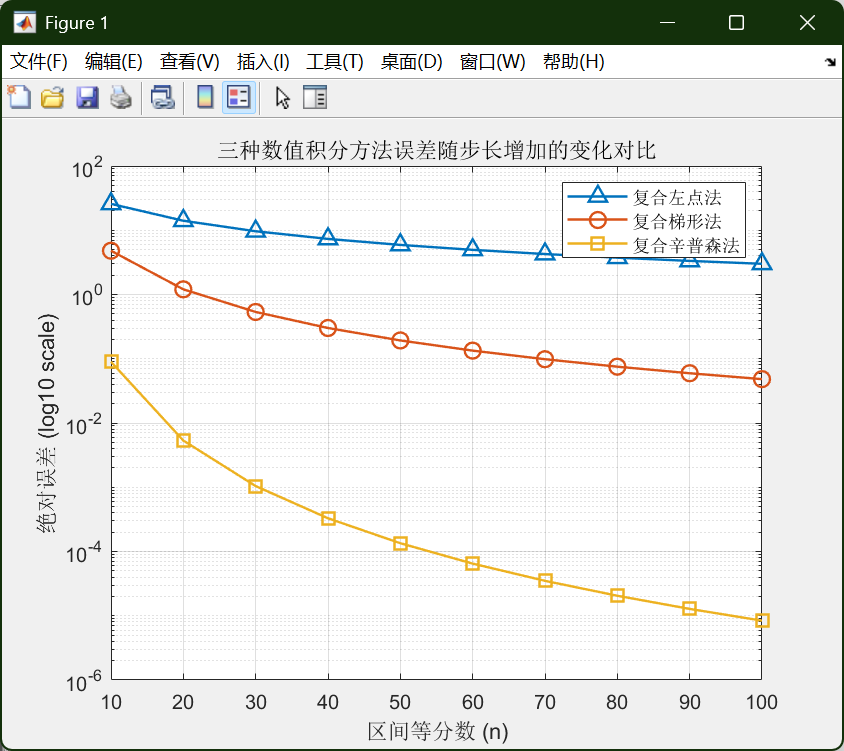
\includegraphics[width=0.9\linewidth]{pic/prb1.png}
    \caption{误差对比}
\end{figure}
\end{document}
